\documentclass{beamer}
\usetheme{Warsaw}

\usepackage[utf8]{inputenc}
\usepackage{fancybox}
\usepackage{multimedia} 
\usepackage{subfig}
\usepackage{amsmath}
\usepackage{hyperref}
\usepackage[all]{xy}
\begin{document}


\title[Angewandte Mathematik] % (optional, only for long titles)
{Angewandte Mathematik
\\
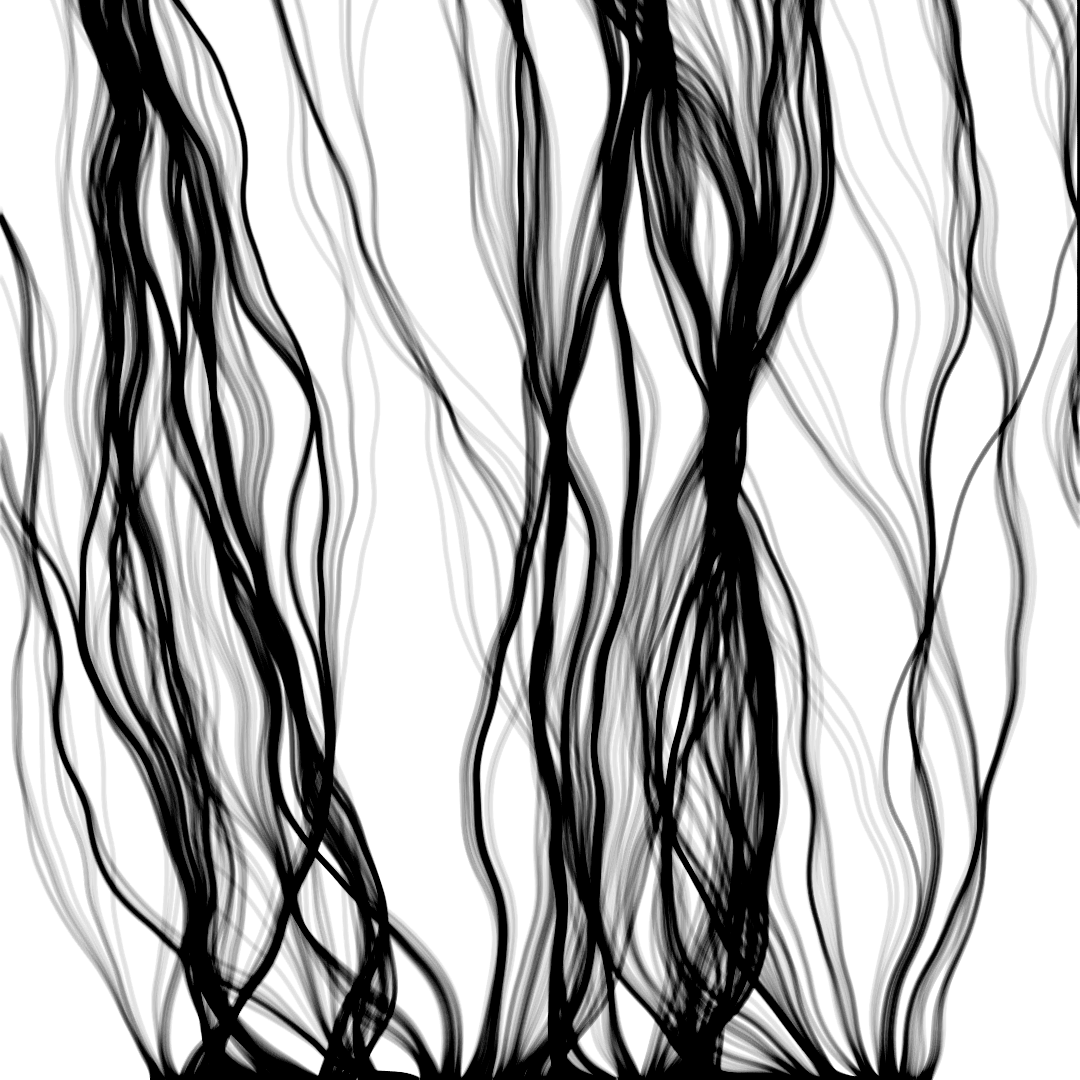
\includegraphics[scale=0.15]{images/cover}
}
\subtitle{}
\author[Dr. Johannes Riesterer] % (optional, for multiple authors)
{Dr.  rer. nat. Johannes Riesterer}

\date[KPT 2004] % (optional)
{}

\subject{Angewandte Mathematik}



\frame{\titlepage}

\begin{frame}
    \frametitle{Angewandte Mathematik}
\framesubtitle{Lebesgue Maß}
    \begin{block}{Wozu Integrieren?}
\begin{itemize}
\item \pause Wie oft muss man ein periodisches Signal Abtasten, um es eindeutig zu rekonstruieren? 
\item \pause  Welchen Anteil hat eine bestimmte Frequenz in einem Signal?
\item \pause Welchen Abstand hat eine  approximierte Funktion zur Original-Funktion? 
\item \pause Filtern von Signalen/Bildern.
\item \pause Probleme so umformulieren, dass man sie besser lösen kann. 
\end{itemize}
\end{block}
 \end{frame}





\begin{frame}
    \frametitle{Angewandte Mathematik}
\framesubtitle{Lebesgue Maß}
    \begin{block}{Wie kann man Inhalte messen?}
Archimedes approximierte den Flächeninhalt einer Kreisscheibe durch Vielecke, deren Flächeninhalt man leicht berechnen kann (250 v. Chr.).
\begin{align*}
\frac{223}{71} < \pi < \frac{22}{7}
\end{align*}
\begin{figure}[H]
      \centering
    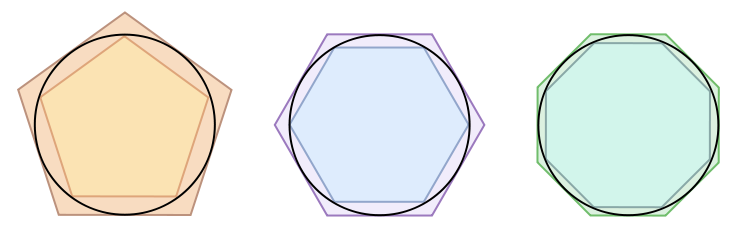
\includegraphics[width=0.7 \textwidth]{images/750px-Archimedes_pi}
      \caption{Quelle: Wikipedia: https://en.wikipedia.org/wiki/File:Archimedes\_pi.svg}
\end{figure}
\end{block}
 \end{frame}



\begin{frame}
    \frametitle{Angewandte Mathematik}
\framesubtitle{Lebesgue Maß}
    \begin{block}{Idee}
\begin{itemize}
\item Überdecke komplizierte Mengen mit einfachen Mengen, deren Inhalt man leicht berechnen kann.
\item \pause Mit Hilfe eines Grenzwertprozesses konstruiert man eine beliebig genaue Überdeckung.
\end{itemize}
\end{block}
\begin{figure}[!tbp]
  \centering
  \begin{minipage}[b]{0.4\textwidth}
    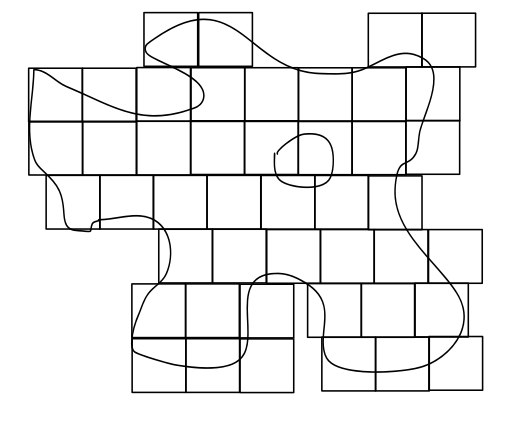
\includegraphics[width=\textwidth]{images/leb1-2}
    \caption{Grobe Überdeckung}
  \end{minipage}
  \hfill
  \begin{minipage}[b]{0.4\textwidth}
    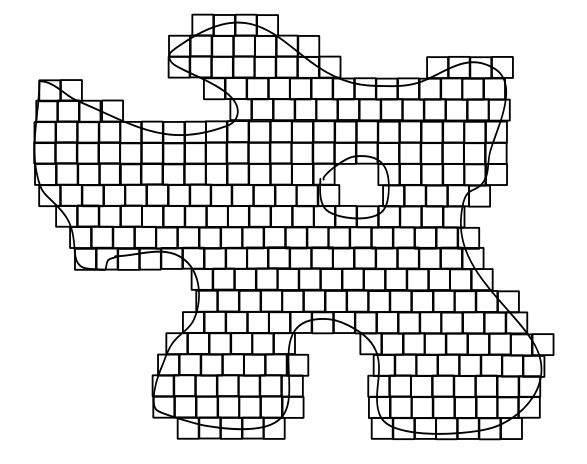
\includegraphics[width=\textwidth]{images/leb2-11}
    \caption{Feinere Überdeckung}
  \end{minipage}
\end{figure}
 \end{frame}





\begin{frame}
    \frametitle{Angewandte Mathematik}
\framesubtitle{Lebesgue Maß}
    \begin{block}{Quader}
Für offene Intervalle $(a_i,b_i) \subset \mathbb{R}$ mit $a_i \leq b_i$ nennen wir 
$$I := (a_1,b_1) \times \cdots \times (a_n,b_n)$$ 
einen $n$-dimensionalen Quader und 
$$\bar{I}:= [a_1, b_1] \times \cdots \times [a_n,b_n]$$
 seinen Abschluss. Wir definieren das Volumen 
\begin{align*}
\text{vol} (I):=   \prod_{i = 1}^n (b_i -a_i)  \; .
\end{align*}

\end{block}
 \end{frame}



\begin{frame}
    \frametitle{Angewandte Mathematik}
\framesubtitle{Lebesgue Maß}
    \begin{block}{Quader}
Mit $$\mathbb{I}(n): = \{   (a_1,b_1) \times \cdots \times (a_n,b_n) \; | \;  (a_i, b_i) \subset \mathbb{R} \}$$ bezeichnen wir die Menge aller $n$-dimensionalen Quader. 
\end{block}
    \begin{block}{Hüllquader}
Für eine Menge $A \subset \mathbb{R}^n$ bezeichnen wir eine Menge von Quadern $\{ I_j \; | \;  I_j \in \mathbf{I}(n)  \}$ mit $A \subset \bigcup_j I_j$ als Hüllquader für $A$.
\end{block}
 \end{frame}


\begin{frame}
    \frametitle{Angewandte Mathematik}
\framesubtitle{Lebesgue Maß}
    \begin{block}{ Lebesguesche äußere Maß}
Für eine Menge $A \subset \mathbb{R}^n$ definieren wir das Lebesguesche äußere Maß durch 
\begin{align*}
\mu (A):=   \inf \biggl \{ \sum_{j=1}^{\infty}   \text{vol} (I_j)\; ; \; I_j \in \mathbb{I}(n); A \subset \bigcup_{j= 1}^{\infty} I_j \biggr \} 
\end{align*}
\end{block}
    \begin{block}{Infimum}
Größte untere Schranke.
\end{block}
 \end{frame}

\begin{frame}
    \frametitle{Angewandte Mathematik}

\begin{figure}[H]
      \centering
    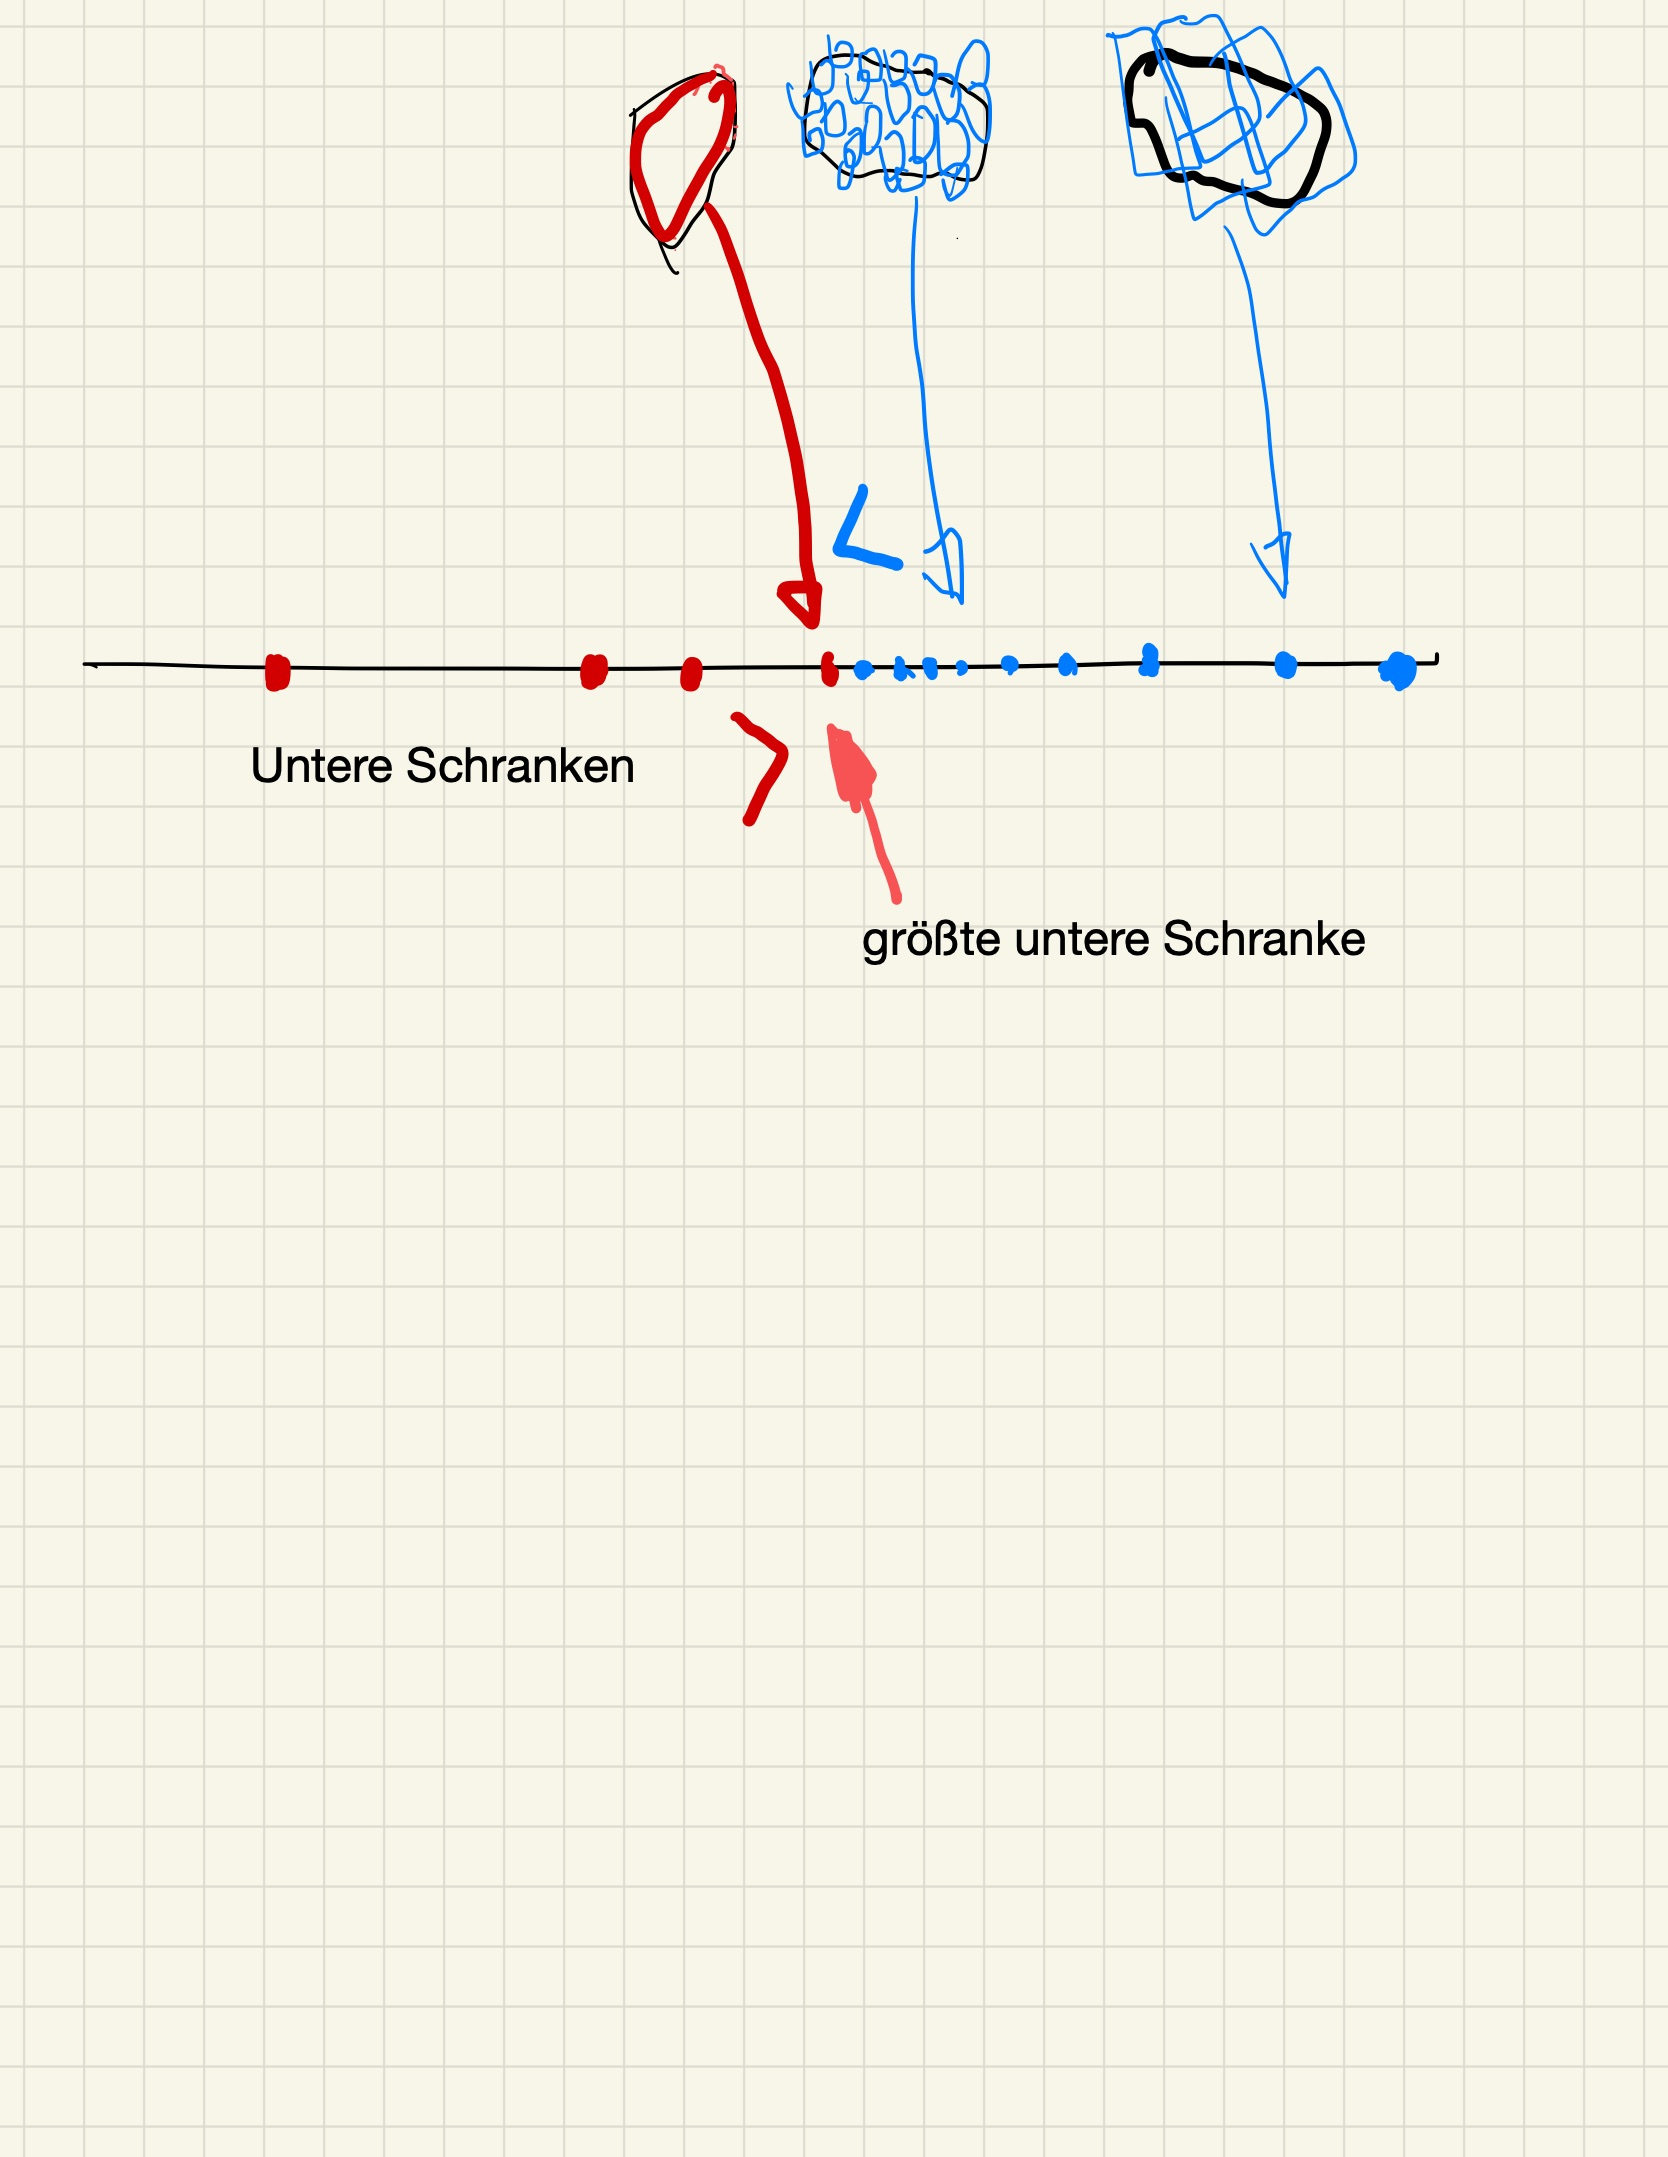
\includegraphics[width=0.8 \textwidth]{notes/untereschranke}
      \caption{}
\end{figure}
 \end{frame}



\begin{frame}
    \frametitle{Angewandte Mathematik}
\framesubtitle{Lebesgue Maß}
    \begin{block}{Monotonie}
Für $A \subset B \subset \mathbb{R}^n$ ist $\mu(A) \leq B$.
\end{block}

    \begin{block}{Beweis}
Da $A \subset B$ Teilmenge ist, sind Hüllquader von $B$  auch Hüllquader von $A$ und damit  $\mu(A) \leq \mu(B)$.
\end{block}
 \end{frame}


\begin{frame}
    \frametitle{Angewandte Mathematik}
\framesubtitle{Lebesgue Maß}
    \begin{block}{$\sigma$-subadditivität}
Sei $A_j \subset \mathbb{R}^n$ eine Folge von Mengen. Dann gilt
\begin{align*}
\mu (\bigcup_j^{\infty} A_j ) \leq \sum_{i=1}^{\infty} \mu(A_j)
\end{align*}
\end{block}
 \end{frame}


\begin{frame}
    \frametitle{Angewandte Mathematik}
\framesubtitle{Lebesgue Maß}
    \begin{block}{}
Für jedes $A_j$ und $\epsilon > 0$ können wir  eine geeignete Überdeckung  $A_j \subset \bigcup_k  K_{j,k}$ mit Hüllquadern $K_{j,k}$ finden, so dass 
 $\sum_k \text{vol} (K_{j,k}) \leq \mu(A) + \frac{\epsilon}{2^{j+1}}$.
Da $ \bigcup_j A_j \subset \bigcup_j \bigcup_k  K_{j,k}$ eine Überdeckung mit Hüllquadern ist, folgt
\begin{align*}
\mu \biggl (  \bigcup A_j  \biggr) & \leq \sum_j \sum_k \text{vol} (K_{j,k}) \leq  \bigl( \sum_j  \mu(A_j) + \frac{\epsilon}{2^{j+1}} \bigr)  \\
&= \bigl (\sum_j \mu(A_j) \bigr ) + \epsilon
\end{align*}
(Die letzte Gleichung beruht auf dem Wert der \href{https://de.wikipedia.org/wiki/Geometrische_Reihe}{geometrischen Reihe}).
Da die letzte Aussage für beliebiges $\epsilon > 0$ gilt, folgt die Behauptung.
\end{block}
 \end{frame}

\end{document}

